% Options for packages loaded elsewhere
\PassOptionsToPackage{unicode}{hyperref}
\PassOptionsToPackage{hyphens}{url}
\PassOptionsToPackage{dvipsnames,svgnames,x11names}{xcolor}
%
\documentclass[
  letterpaper,
  DIV=11,
  numbers=noendperiod]{scrreprt}

\usepackage{amsmath,amssymb}
\usepackage{iftex}
\ifPDFTeX
  \usepackage[T1]{fontenc}
  \usepackage[utf8]{inputenc}
  \usepackage{textcomp} % provide euro and other symbols
\else % if luatex or xetex
  \usepackage{unicode-math}
  \defaultfontfeatures{Scale=MatchLowercase}
  \defaultfontfeatures[\rmfamily]{Ligatures=TeX,Scale=1}
\fi
\usepackage{lmodern}
\ifPDFTeX\else  
    % xetex/luatex font selection
\fi
% Use upquote if available, for straight quotes in verbatim environments
\IfFileExists{upquote.sty}{\usepackage{upquote}}{}
\IfFileExists{microtype.sty}{% use microtype if available
  \usepackage[]{microtype}
  \UseMicrotypeSet[protrusion]{basicmath} % disable protrusion for tt fonts
}{}
\makeatletter
\@ifundefined{KOMAClassName}{% if non-KOMA class
  \IfFileExists{parskip.sty}{%
    \usepackage{parskip}
  }{% else
    \setlength{\parindent}{0pt}
    \setlength{\parskip}{6pt plus 2pt minus 1pt}}
}{% if KOMA class
  \KOMAoptions{parskip=half}}
\makeatother
\usepackage{xcolor}
\setlength{\emergencystretch}{3em} % prevent overfull lines
\setcounter{secnumdepth}{1}
% Make \paragraph and \subparagraph free-standing
\ifx\paragraph\undefined\else
  \let\oldparagraph\paragraph
  \renewcommand{\paragraph}[1]{\oldparagraph{#1}\mbox{}}
\fi
\ifx\subparagraph\undefined\else
  \let\oldsubparagraph\subparagraph
  \renewcommand{\subparagraph}[1]{\oldsubparagraph{#1}\mbox{}}
\fi


\providecommand{\tightlist}{%
  \setlength{\itemsep}{0pt}\setlength{\parskip}{0pt}}\usepackage{longtable,booktabs,array}
\usepackage{calc} % for calculating minipage widths
% Correct order of tables after \paragraph or \subparagraph
\usepackage{etoolbox}
\makeatletter
\patchcmd\longtable{\par}{\if@noskipsec\mbox{}\fi\par}{}{}
\makeatother
% Allow footnotes in longtable head/foot
\IfFileExists{footnotehyper.sty}{\usepackage{footnotehyper}}{\usepackage{footnote}}
\makesavenoteenv{longtable}
\usepackage{graphicx}
\makeatletter
\def\maxwidth{\ifdim\Gin@nat@width>\linewidth\linewidth\else\Gin@nat@width\fi}
\def\maxheight{\ifdim\Gin@nat@height>\textheight\textheight\else\Gin@nat@height\fi}
\makeatother
% Scale images if necessary, so that they will not overflow the page
% margins by default, and it is still possible to overwrite the defaults
% using explicit options in \includegraphics[width, height, ...]{}
\setkeys{Gin}{width=\maxwidth,height=\maxheight,keepaspectratio}
% Set default figure placement to htbp
\makeatletter
\def\fps@figure{htbp}
\makeatother

\KOMAoption{captions}{tableheading}
\makeatletter
\makeatother
\makeatletter
\@ifpackageloaded{bookmark}{}{\usepackage{bookmark}}
\makeatother
\makeatletter
\@ifpackageloaded{caption}{}{\usepackage{caption}}
\AtBeginDocument{%
\ifdefined\contentsname
  \renewcommand*\contentsname{Içindekiler}
\else
  \newcommand\contentsname{Içindekiler}
\fi
\ifdefined\listfigurename
  \renewcommand*\listfigurename{Şekil Listesi}
\else
  \newcommand\listfigurename{Şekil Listesi}
\fi
\ifdefined\listtablename
  \renewcommand*\listtablename{Tablo Listesi}
\else
  \newcommand\listtablename{Tablo Listesi}
\fi
\ifdefined\figurename
  \renewcommand*\figurename{Figür}
\else
  \newcommand\figurename{Figür}
\fi
\ifdefined\tablename
  \renewcommand*\tablename{Tablo}
\else
  \newcommand\tablename{Tablo}
\fi
}
\@ifpackageloaded{float}{}{\usepackage{float}}
\floatstyle{ruled}
\@ifundefined{c@chapter}{\newfloat{codelisting}{h}{lop}}{\newfloat{codelisting}{h}{lop}[chapter]}
\floatname{codelisting}{Listeleme}
\newcommand*\listoflistings{\listof{codelisting}{İlan Listesi}}
\makeatother
\makeatletter
\@ifpackageloaded{caption}{}{\usepackage{caption}}
\@ifpackageloaded{subcaption}{}{\usepackage{subcaption}}
\makeatother
\makeatletter
\makeatother
\ifLuaTeX
\usepackage[bidi=basic]{babel}
\else
\usepackage[bidi=default]{babel}
\fi
\babelprovide[main,import]{turkish}
% get rid of language-specific shorthands (see #6817):
\let\LanguageShortHands\languageshorthands
\def\languageshorthands#1{}
\ifLuaTeX
  \usepackage{selnolig}  % disable illegal ligatures
\fi
\IfFileExists{bookmark.sty}{\usepackage{bookmark}}{\usepackage{hyperref}}
\IfFileExists{xurl.sty}{\usepackage{xurl}}{} % add URL line breaks if available
\urlstyle{same} % disable monospaced font for URLs
\hypersetup{
  pdftitle={Patoloji Atlası},
  pdfauthor={Serdar Balcı; Patoloji Hekim ve Teknikerleri},
  pdflang={tr},
  colorlinks=true,
  linkcolor={blue},
  filecolor={Maroon},
  citecolor={Blue},
  urlcolor={Blue},
  pdfcreator={LaTeX via pandoc}}

\title{Patoloji Atlası}
\usepackage{etoolbox}
\makeatletter
\providecommand{\subtitle}[1]{% add subtitle to \maketitle
  \apptocmd{\@title}{\par {\large #1 \par}}{}{}
}
\makeatother
\subtitle{Patoloji Atlası: Tıp Fakültesi ve Sağlık Bilimleri Öğrencileri
İçin Patoloji Laboratuvar Notları: Görerek Öğrenin}
\author{Serdar Balcı \and Patoloji Hekim ve Teknikerleri}
\date{2023-09-15}

\begin{document}
\maketitle
\begin{abstract}
Patoloji Atlası: Tıp Fakültesi ve Sağlık Bilimleri Öğrencileri İçin
Patoloji Laboratuvar Notları. Görerek Öğrenin. Patoloji Atlası Memorial
Patoloji arşivinden derlenen vakalardan ve diğer kurumlardan katkı yapan
meslektaşlarımızın kolleksiyonlarından oluşmaktadır. Katkı yapmak ve
kendi vakalarınız ekletmek için lütfen
\href{https://www.patolojiatlasi.com/katki.html}{iletişime geçin}.
\end{abstract}
\renewcommand*\contentsname{İçindekiler}
{
\hypersetup{linkcolor=}
\setcounter{tocdepth}{1}
\tableofcontents
}
\bookmarksetup{startatroot}

\chapter*{Patoloji Atlası}\label{sec-patoloji-atlasi}
\addcontentsline{toc}{chapter}{Patoloji Atlası}

\markboth{Patoloji Atlası}{Patoloji Atlası}

\begin{itemize}
\item
  For English \href{https://www.histopathologyatlas.com/}{click here}.
\item
  Sosyal medyadan derlenen görüntülerden oluşan patoloji notları için
  \href{https://www.patolojinotlari.com/}{tıklayın}.\\
\end{itemize}

\bookmarksetup{startatroot}

\chapter*{Giriş}\label{sec-giris}
\addcontentsline{toc}{chapter}{Giriş}

\markboth{Giriş}{Giriş}

Patoloji Atlası Memorial Patoloji arşivinden ve diğer kurumlardan katkı
yapan meslektaşlarımızın koleksiyonlarından oluşmaktadır.

\href{https://www.patolojiatlasi.com/katki.html}{Katkı yapmak ve kendi
vakalarınız ekletmek için lütfen iletişime geçin}.

\begin{verbatim}
Son güncelleme zamanı: 2023-09-15 17:41:54
\end{verbatim}

Sosyal medyadan derlenen görüntülerden oluşan
\href{https://www.patolojinotlari.com/}{patoloji notları için
tıklayınız}.

\part{Genel Patoloji}

\chapter{Patolojide Kullanılan
Teknikler}\label{sec-patolojide-kullanilan-teknikler}

\section{Histokimya}\label{sec-histokimya}

\subsection{Müsin}\label{sec-musin}

\subsubsection{Mucicarmine}\label{sec-mucicarmine}

\textbf{Normal kolon mukozasında intrasitoplazmik müsini gösteren
mucicarmine (müsikarmen) histokimyası}


\includegraphics[width=0.15\textwidth,height=\textheight]{index_files/mediabag/qrcodes/mucicarmine_qrcode.pdf}
\href{https://images.patolojiatlasi.com/mucin/mucicarmine.html}{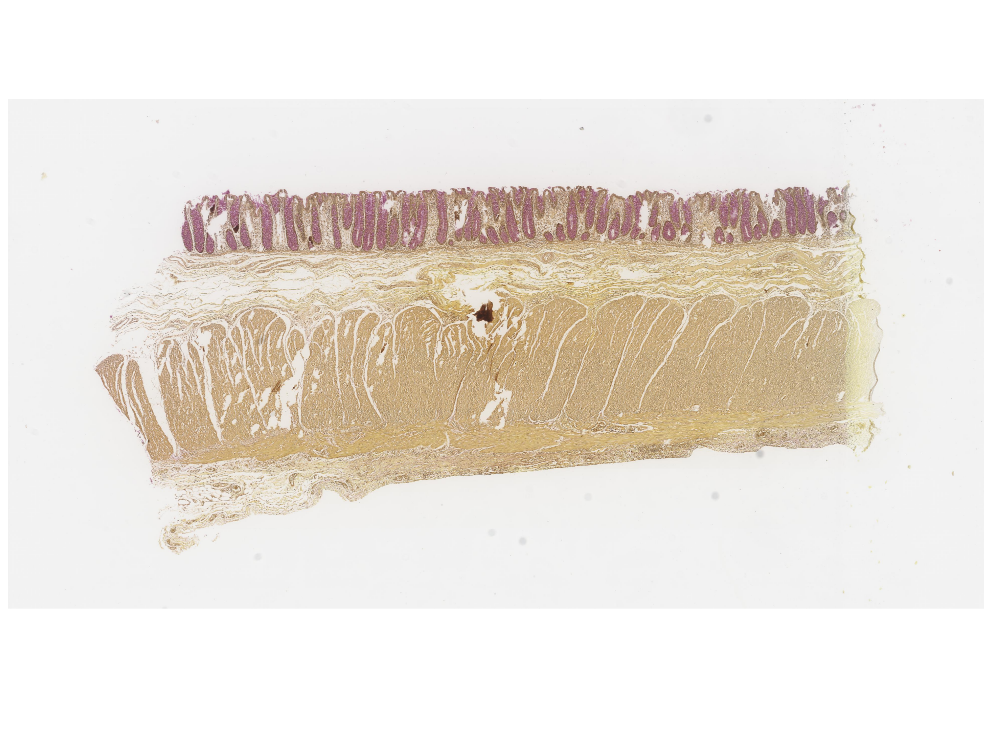
\includegraphics[width=0.25\textwidth,height=\textheight]{./screenshots/thumbnail_mucicarmine.png}}
\href{https://images.patolojiatlasi.com/mucin/mucicarmine.html}{Tam
Ekran Görmek İçin Resmi Tıklayın}

\section{Chromogenic in situ hybridization
(CISH)}\label{sec-chromogenic-in-situ-hybridization-cish}

\textbf{Chromogenic in situ hybridization (CISH)}


\includegraphics[width=0.15\textwidth,height=\textheight]{index_files/mediabag/qrcodes/cish_qrcode.pdf}
\href{https://images.patolojiatlasi.com/her2-cish/cish.html}{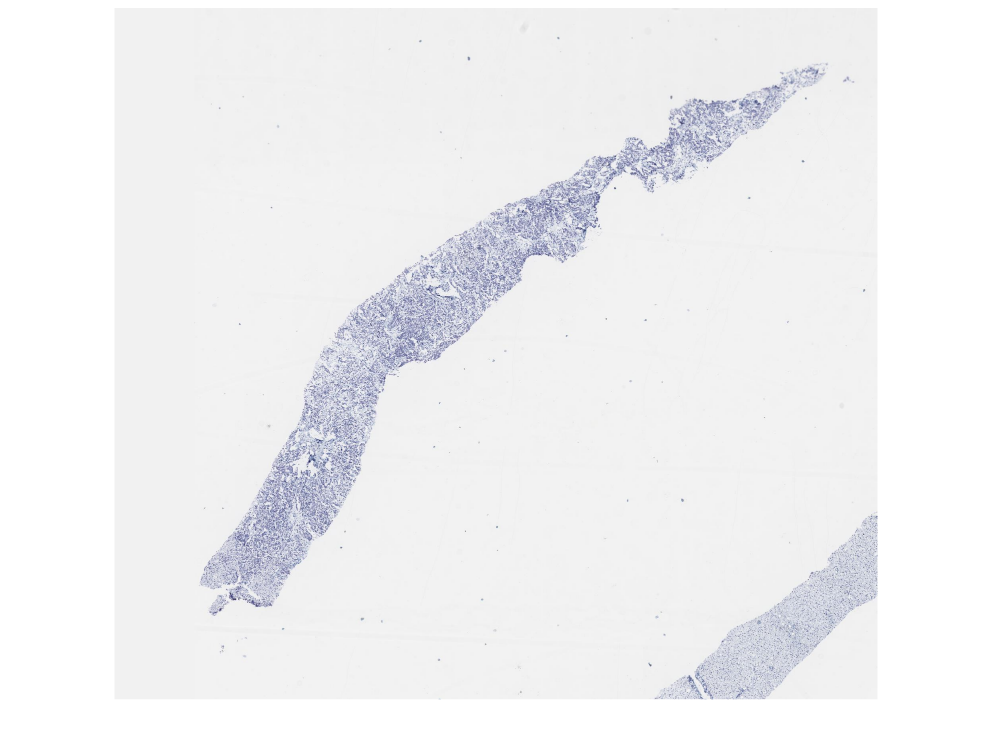
\includegraphics[width=0.25\textwidth,height=\textheight]{./screenshots/thumbnail_cish.png}}
\href{https://images.patolojiatlasi.com/her2-cish/cish.html}{Tam Ekran
Görmek İçin Resmi Tıklayın}

\chapter{Hücre İçi Birikimler}\label{sec-hucre-ici-birikimler}

\section{Kolesterol Polibi}\label{sec-kolesterol-polibi}

\textbf{Kolesterol Polibi}

\href{https://images.patolojiatlasi.com/cholesterolpolyp/HE.html}{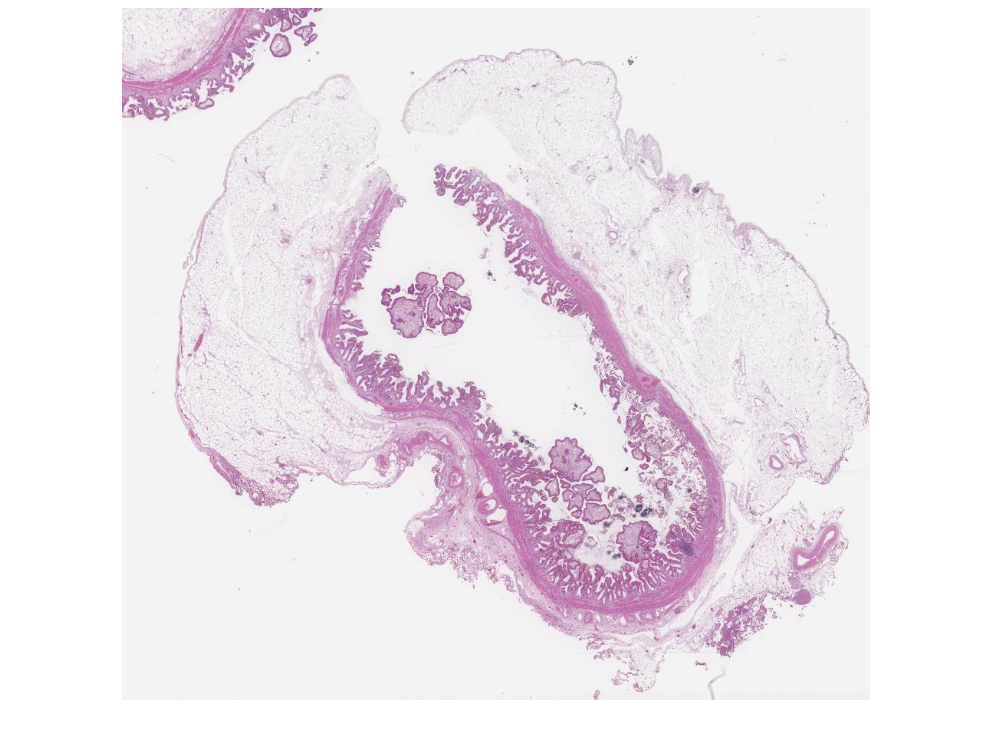
\includegraphics[width=0.25\textwidth,height=\textheight]{./screenshots/thumbnail_cholesterolpolyp.png}}
\href{https://images.patolojiatlasi.com/cholesterolpolyp/HE.html}{Tam
Ekran Görmek İçin Resmi Tıklayın}

\section{Glikojen Depo Hastalığı}\label{sec-glikojen-depo-hastaligi}

\subsection{HE}\label{he}

\textbf{Karaciğer İğnde Biyopsisinde glikojen depo hastalığı}

\textbf{Hematoksilen Eozin}


\includegraphics[width=0.15\textwidth,height=\textheight]{index_files/mediabag/qrcodes/glycogenstorage-HE_qrcode.pdf}
\href{https://images.patolojiatlasi.com/glycogenstorage/HE.html}{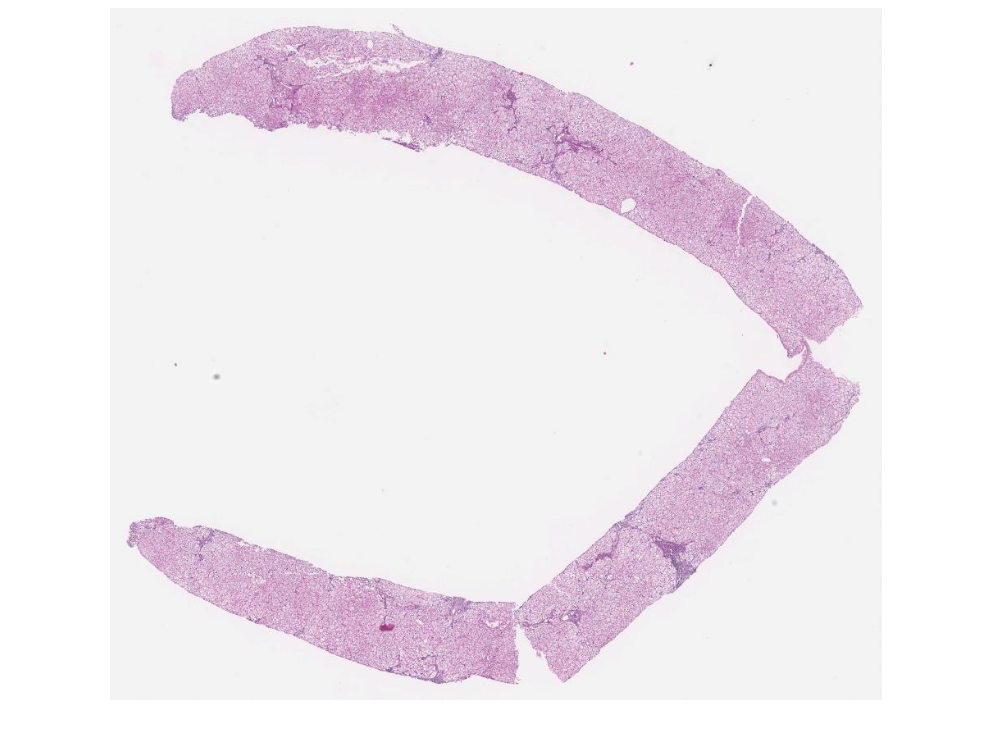
\includegraphics[width=0.25\textwidth,height=\textheight]{./screenshots/thumbnail_glycogenstorage-HE.png}}
\href{https://images.patolojiatlasi.com/glycogenstorage/HE.html}{Tam
Ekran Görmek İçin Resmi Tıklayın}

\subsection{PAS}\label{pas}

\textbf{PAS}


\includegraphics[width=0.15\textwidth,height=\textheight]{index_files/mediabag/qrcodes/glycogenstorage-PAS_qrcode.pdf}
\href{https://images.patolojiatlasi.com/glycogenstorage/PAS.html}{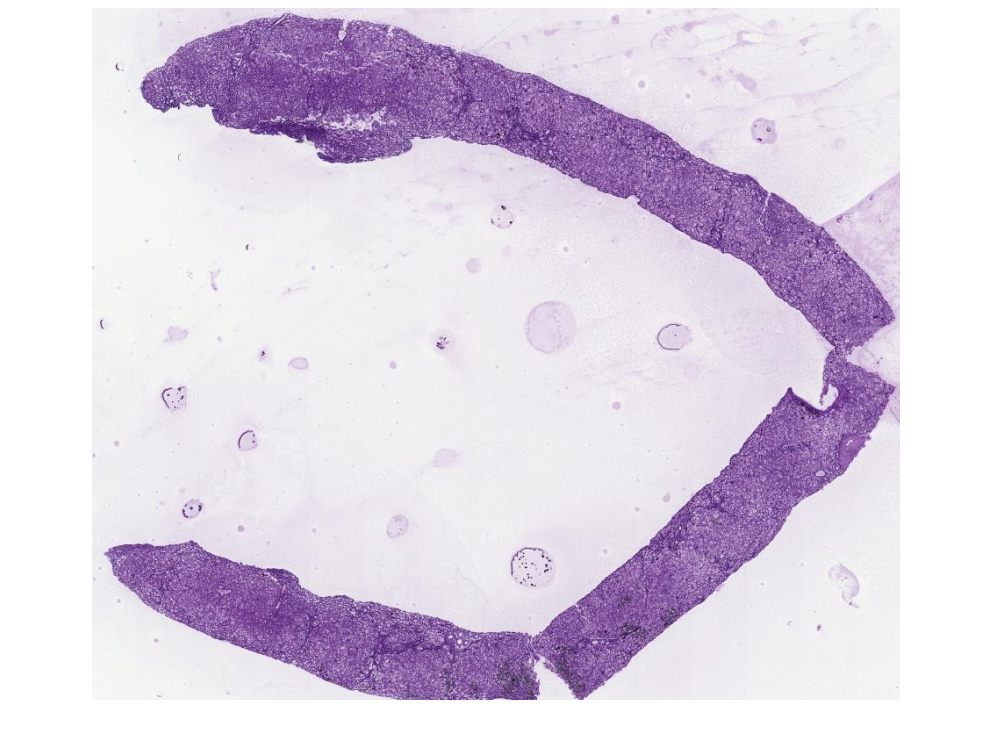
\includegraphics[width=0.25\textwidth,height=\textheight]{./screenshots/thumbnail_glycogenstorage-PAS.png}}
\href{https://images.patolojiatlasi.com/glycogenstorage/PAS.html}{Tam
Ekran Görmek İçin Resmi Tıklayın}

\subsection{PASD}\label{pasd}

\textbf{PASD}


\includegraphics[width=0.15\textwidth,height=\textheight]{index_files/mediabag/qrcodes/glycogenstorage-PASD_qrcode.pdf}
\href{https://images.patolojiatlasi.com/glycogenstorage/PASD.html}{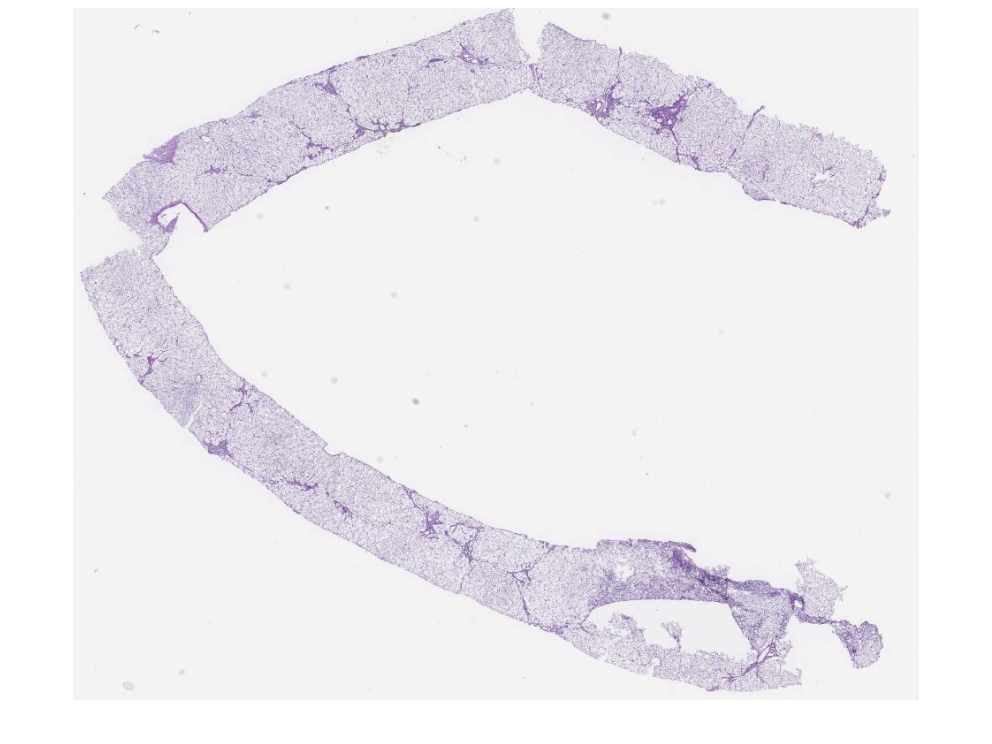
\includegraphics[width=0.25\textwidth,height=\textheight]{./screenshots/thumbnail_glycogenstorage-PASD.png}}
\href{https://images.patolojiatlasi.com/glycogenstorage/PASD.html}{Tam
Ekran Görmek İçin Resmi Tıklayın}

\section{Antrakoz, Antrakotik
Pigment}\label{sec-antrakoz-antrakotik-pigment}

Torakal bölge lenf nodunda antrakotik pigment

\subsubsection{HE-1}\label{he-1}


\includegraphics[width=0.15\textwidth,height=\textheight]{index_files/mediabag/qrcodes/anthracosis-HE1_qrcode.pdf}
\href{https://images.patolojiatlasi.com/anthracosis/HE.html}{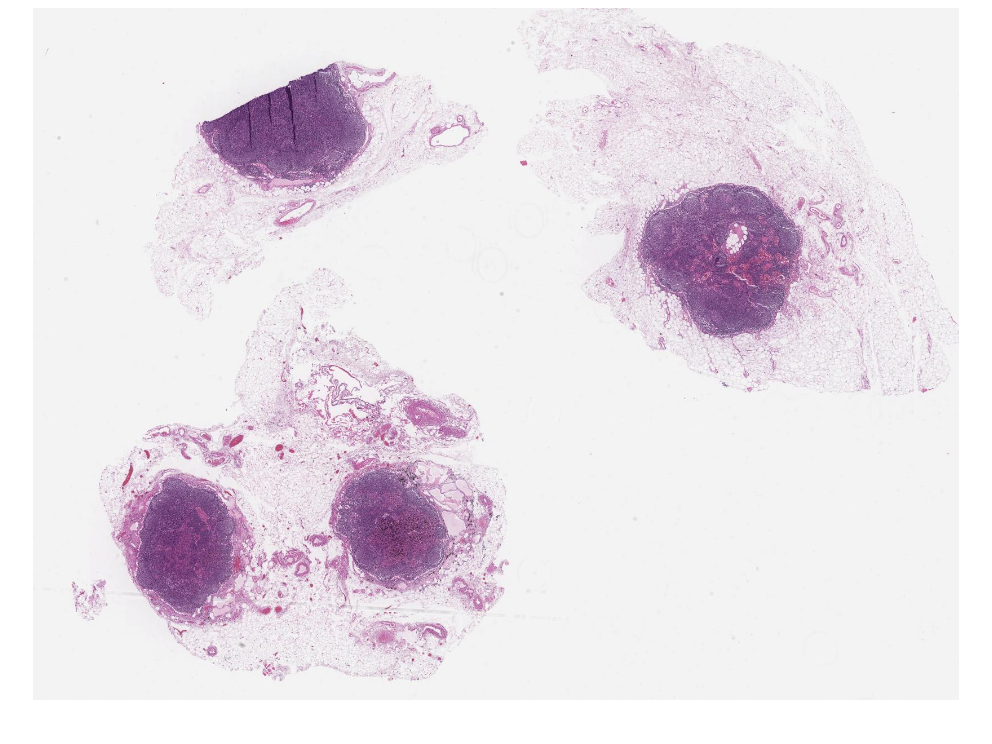
\includegraphics[width=0.25\textwidth,height=\textheight]{./screenshots/thumbnail_anthracosis1.png}}
\href{https://images.patolojiatlasi.com/anthracosis/HE.html}{Click for
Full Screen WSI}

\subsubsection{HE-2}\label{he-2}


\includegraphics[width=0.15\textwidth,height=\textheight]{index_files/mediabag/qrcodes/anthracosis-HE2_qrcode.pdf}
\href{https://images.patolojiatlasi.com/anthracosis/HE2.html}{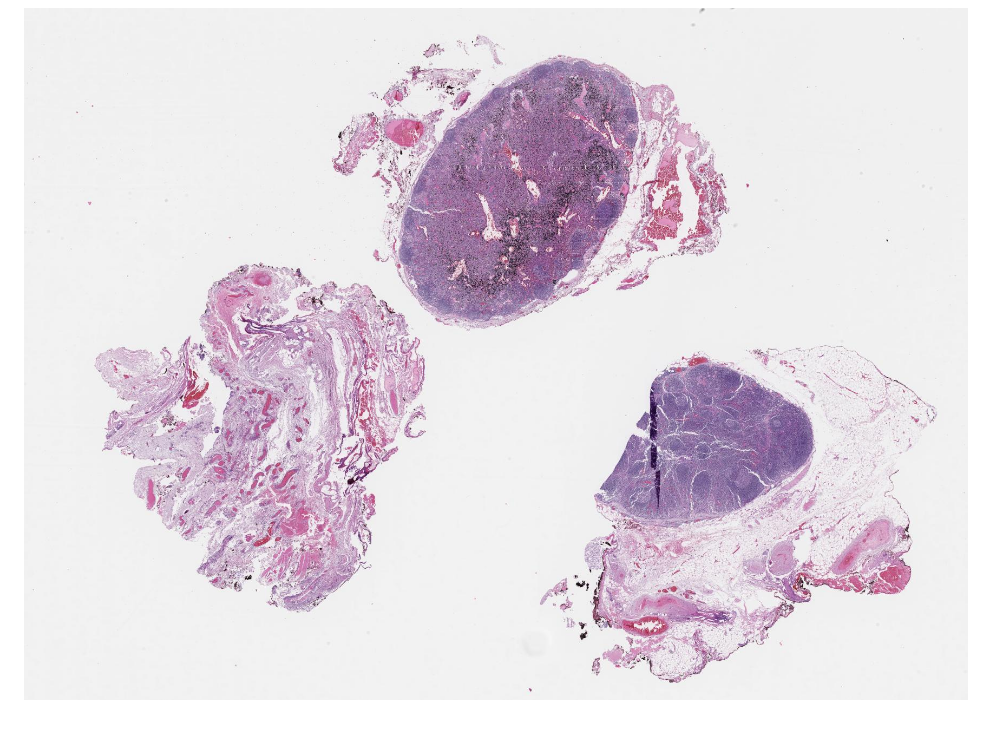
\includegraphics[width=0.25\textwidth,height=\textheight]{./screenshots/thumbnail_anthracosis2.png}}
\href{https://images.patolojiatlasi.com/anthracosis/HE2.html}{Click for
Full Screen WSI}

\subsubsection{HE-1}\label{he-1-1}

\subsubsection{HE-2}\label{he-2-1}

\section{Melanosis Coli}\label{sec-melanosis-coli}

::: \{.\}

\subsection{HE}\label{he-3}

\textbf{Melanozis Koli}


\includegraphics[width=0.15\textwidth,height=\textheight]{index_files/mediabag/qrcodes/melanosiscoli-HE_qrcode.pdf}
\href{https://images.patolojiatlasi.com/melanosiscoli/HE.html}{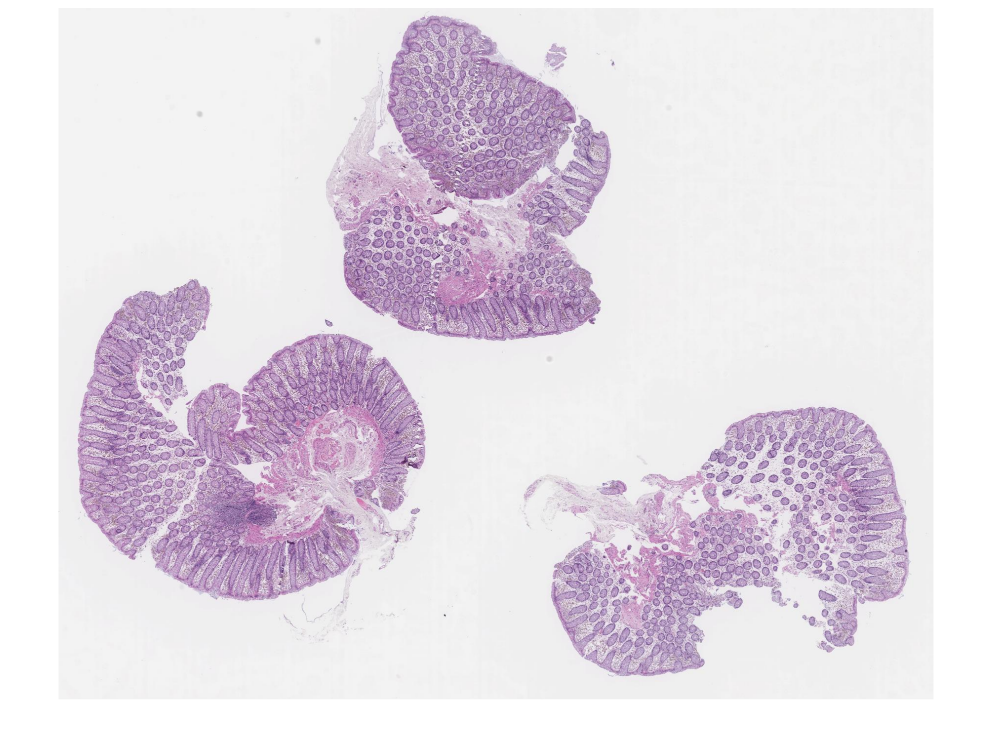
\includegraphics[width=0.25\textwidth,height=\textheight]{./screenshots/thumbnail_melanosiscoli-HE.png}}
\href{https://images.patolojiatlasi.com/melanosiscoli/HE.html}{Tam Ekran
Görmek İçin Resmi Tıklayın}

\subsection{PAS}\label{pas-1}

\textbf{Melanozis Koli PAS}


\includegraphics[width=0.15\textwidth,height=\textheight]{index_files/mediabag/qrcodes/melanosiscoli-PAS_qrcode.pdf}
\href{https://images.patolojiatlasi.com/melanosiscoli/PAS.html}{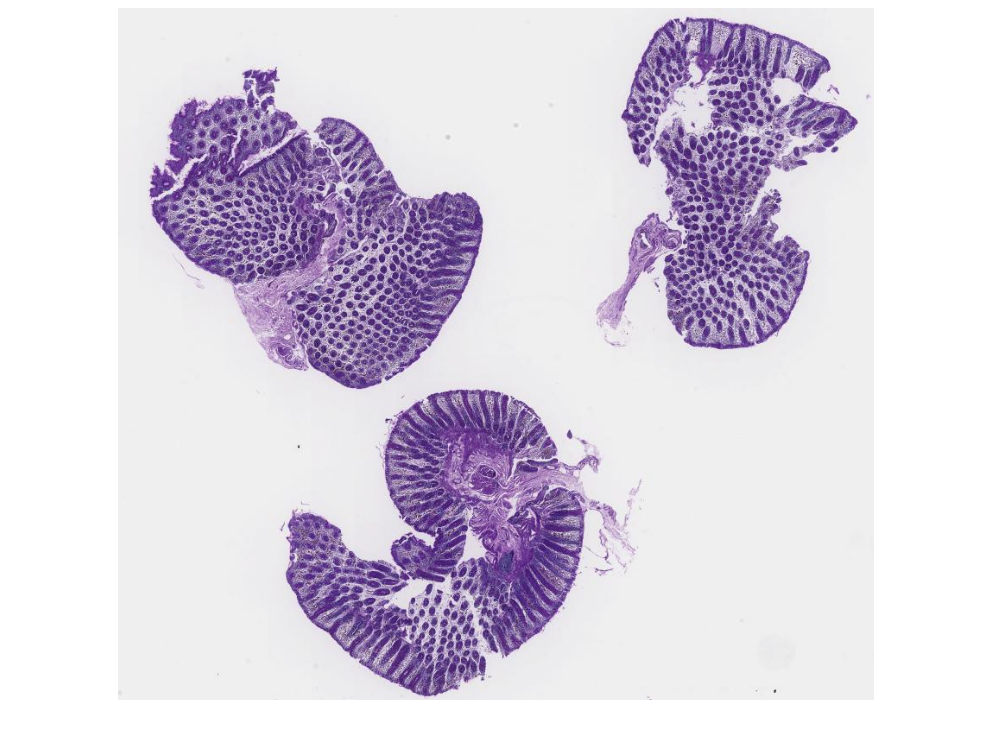
\includegraphics[width=0.25\textwidth,height=\textheight]{./screenshots/thumbnail_melanosiscoli-PAS.png}}
\href{https://images.patolojiatlasi.com/melanosiscoli/PAS.html}{Tam
Ekran Görmek İçin Resmi Tıklayın}

\chapter{Hücre Dışı Birikimler}\label{sec-hucre-disi-birikimler}

\section{Okronozis}\label{sec-okronozis}

\textbf{Okronozis}


\includegraphics[width=0.15\textwidth,height=\textheight]{index_files/mediabag/qrcodes/ochronosis-HE_qrcode.pdf}
\href{https://images.patolojiatlasi.com/ochronosis/HE.html}{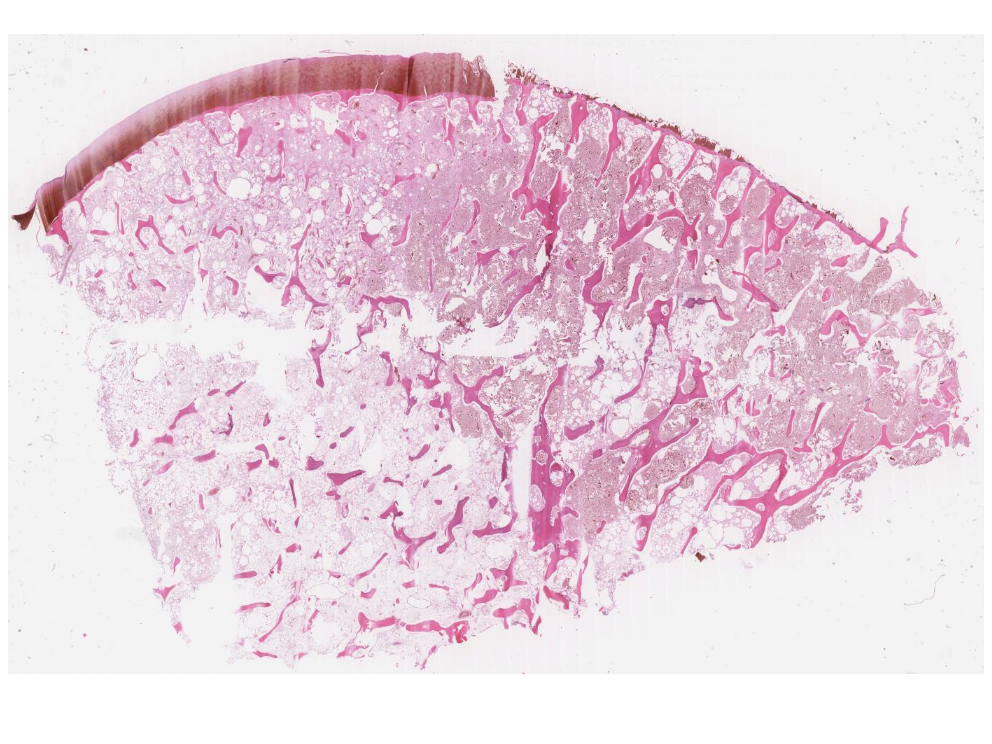
\includegraphics[width=0.25\textwidth,height=\textheight]{./screenshots/thumbnail_ochronosis.png}}
\href{https://images.patolojiatlasi.com/ochronosis/HE.html}{Tam Ekran
Görmek İçin Resmi Tıklayın}

\chapter{Hücre Hasarı}\label{sec-hucre-hasari}

\section{Reaktif Atipi, ülsere kolon polibi}\label{sec-reaktif-atipi}

\textbf{Reaktif Atipi, ülsere kolon polibi}


\includegraphics[width=0.15\textwidth,height=\textheight]{index_files/mediabag/qrcodes/reactive-atypia-HE_qrcode.pdf}
\href{https://images.patolojiatlasi.com/reactive-atypia/HE.html}{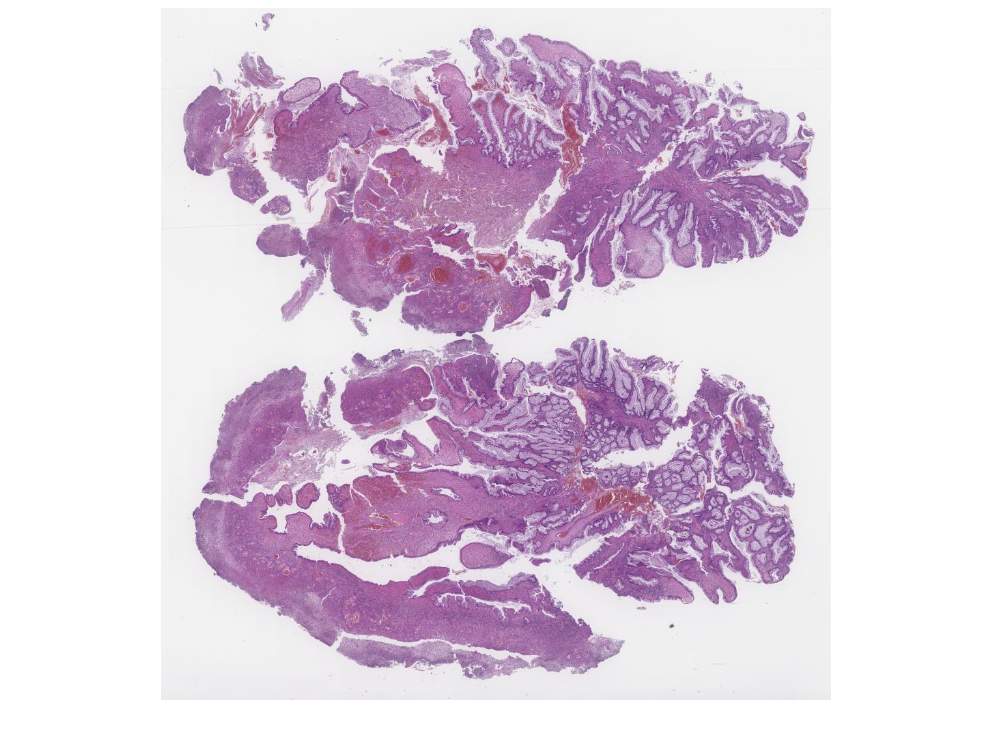
\includegraphics[width=0.25\textwidth,height=\textheight]{./screenshots/thumbnail_reactive-atypia.png}}
\href{https://images.patolojiatlasi.com/reactive-atypia/HE.html}{Tam
Ekran Görmek İçin Resmi Tıklayın}

\chapter{İskemi ve Nekroz}\label{sec-iskemi-ve-nekroz}

\section{Yağ nekrozu ve Sabunlaşma}\label{sec-yag-nekrozu-sabunlasma}


\includegraphics[width=0.15\textwidth,height=\textheight]{index_files/mediabag/qrcodes/fat-necrosis-HE_qrcode.pdf}
\href{https://images.patolojiatlasi.com/fat-necrosis/HE.html}{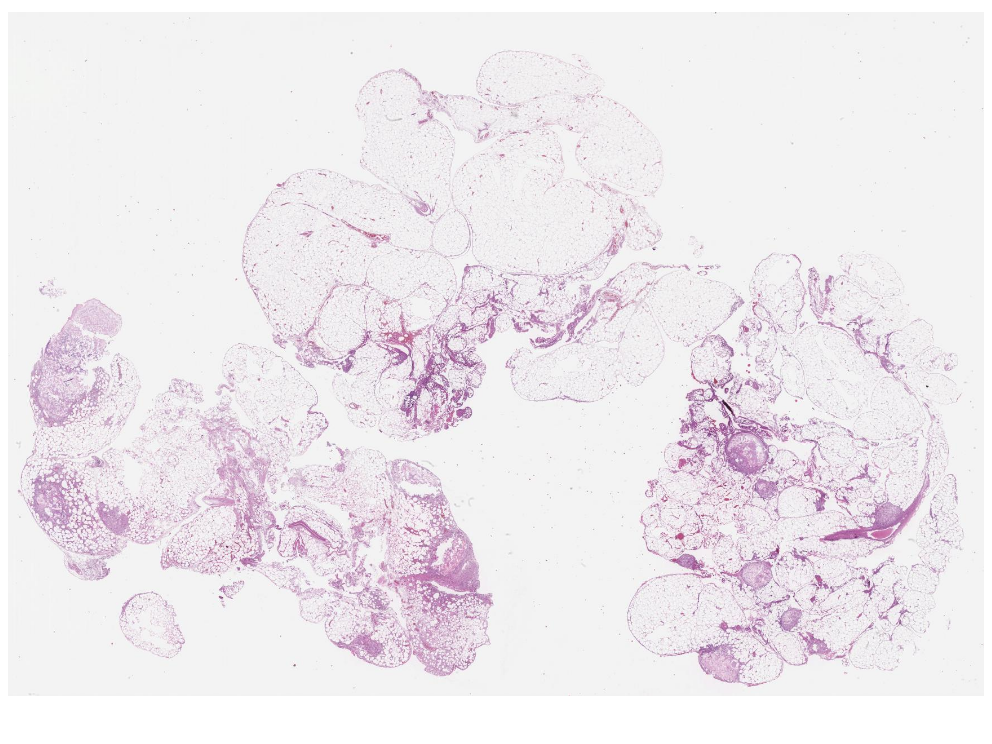
\includegraphics[width=0.25\textwidth,height=\textheight]{./screenshots/thumbnail_fat-necrosis.png}}
\href{https://images.patolojiatlasi.com/fat-necrosis/HE.html}{Tam Ekran
Görmek İçin Resmi Tıklayın}

\chapter{Dalak konjesyon}\label{sec-congestion-spleen}

\textbf{Dalak konjesyon}


\includegraphics[width=0.15\textwidth,height=\textheight]{index_files/mediabag/qrcodes/congestion-spleen-HE_qrcode.pdf}
\href{https://images.patolojiatlasi.com/congestion-spleen/HE.html}{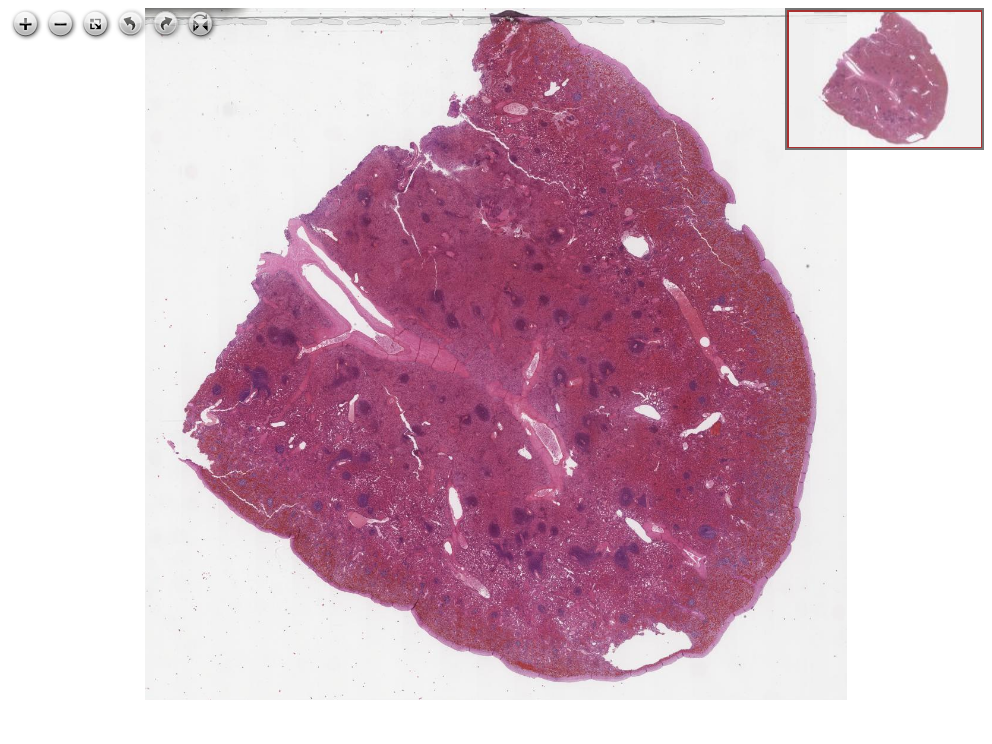
\includegraphics[width=0.25\textwidth,height=\textheight]{./screenshots/thumbnail_congestion-spleen.png}}
\href{https://images.patolojiatlasi.com/congestion-spleen/HE.html}{Tam
Ekran Görmek İçin Resmi Tıklayın}

\chapter{Amiloidoz (Amiloid Birikimi)}\label{sec-amiloidoz}

\section{Kristal Viyole}\label{sec-amiloidoz-kristal-viyole}

\textbf{Damar duvarlarında amiloid birikimi}


\includegraphics[width=0.15\textwidth,height=\textheight]{index_files/mediabag/qrcodes/amyloid-crystalviolet_qrcode.pdf}
\href{https://images.patolojiatlasi.com/amyloid/crystalviolet.html}{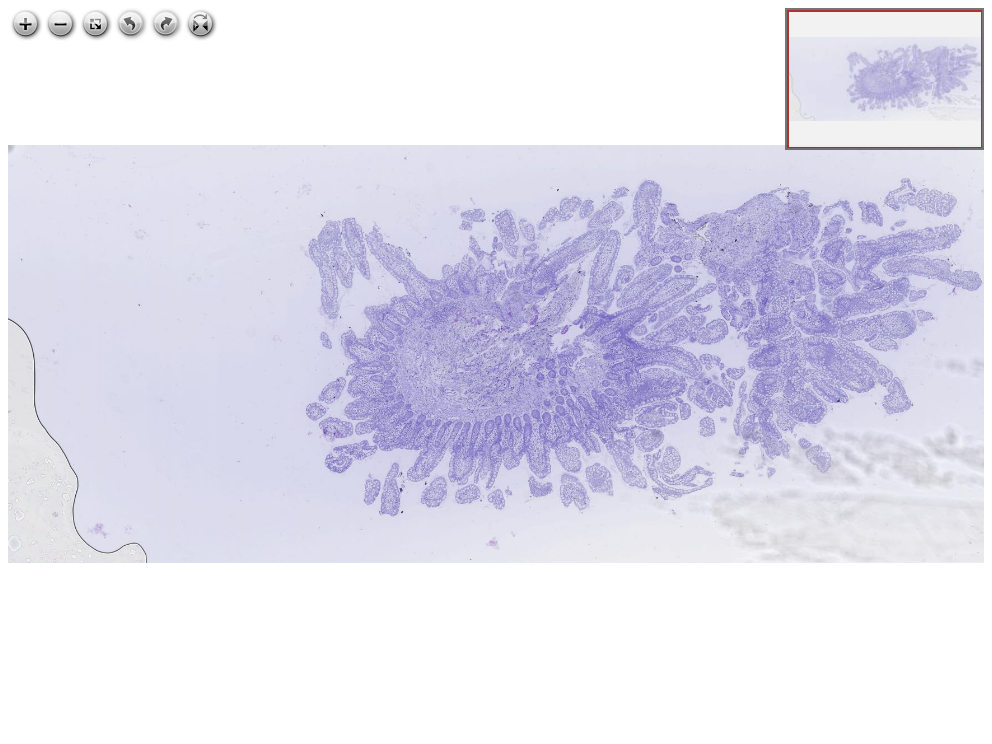
\includegraphics[width=0.25\textwidth,height=\textheight]{./screenshots/thumbnail_crystalviolet.png}}
\href{https://images.patolojiatlasi.com/amyloid/crystalviolet.html}{Tam
Ekran Görmek İçin Resmi Tıklayın}

\section{Kongo Kırmızısı}\label{sec-amiloidoz-kongo-kirmizisi}

\textbf{Congo Red stain for amyloidosis}


\includegraphics[width=0.15\textwidth,height=\textheight]{index_files/mediabag/qrcodes/congored-congored_qrcode.pdf}
\href{https://images.patolojiatlasi.com/congored/congored.html}{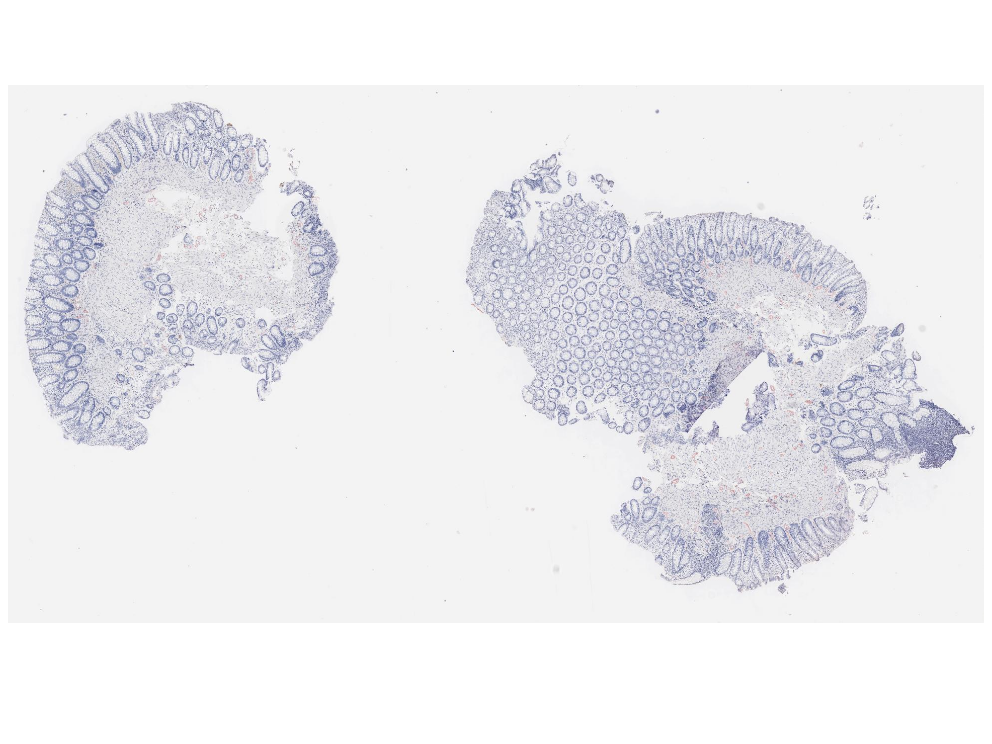
\includegraphics[width=0.25\textwidth,height=\textheight]{./screenshots/thumbnail_congored.png}}
\href{https://images.patolojiatlasi.com/congored/congored.html}{Tam
Ekran Görmek İçin Resmi Tıklayın}

\subsection{Video}\label{video}

\textbf{Kongo Kırmızısı Çift Kırıcılık}

\url{https://www.youtube.com/watch?v=U9glkfQLTm4}

\textbf{Congo Red Birefringence}

\href{https://www.youtube.com/watch?v=U9glkfQLTm4}{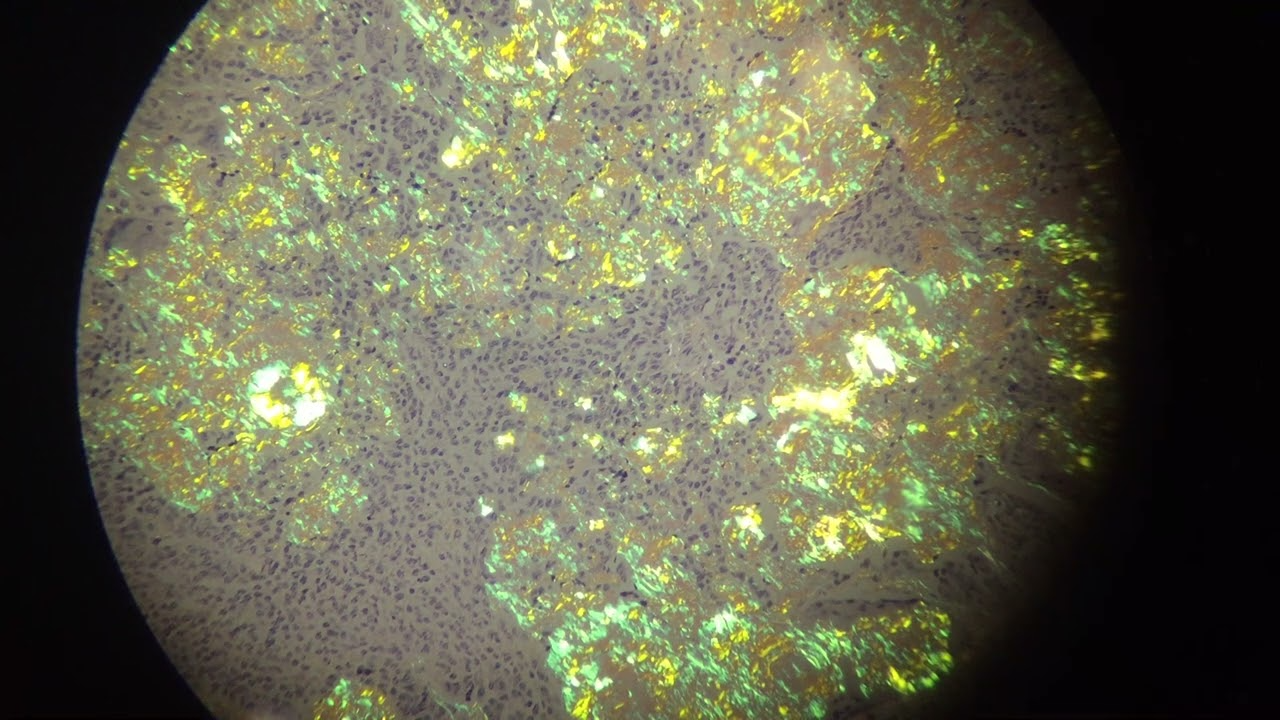
\includegraphics[width=0.25\textwidth,height=\textheight]{./screenshots/thumbnail_congored_video.png}}
\href{https://www.youtube.com/watch?v=U9glkfQLTm4}{Video İçin Tıklayın}

\chapter{Tamir Mekanizmaları}\label{sec-tamir-mekanizmalari}

\section{Fibrozis}\label{sec-fibrozis}

Kolesistit spesmeninde gelişmekte olan genç fibrozis


\includegraphics[width=0.15\textwidth,height=\textheight]{index_files/mediabag/qrcodes/fibrosis-HE_qrcode.pdf}
\href{https://images.patolojiatlasi.com/fibrosis/HE.html}{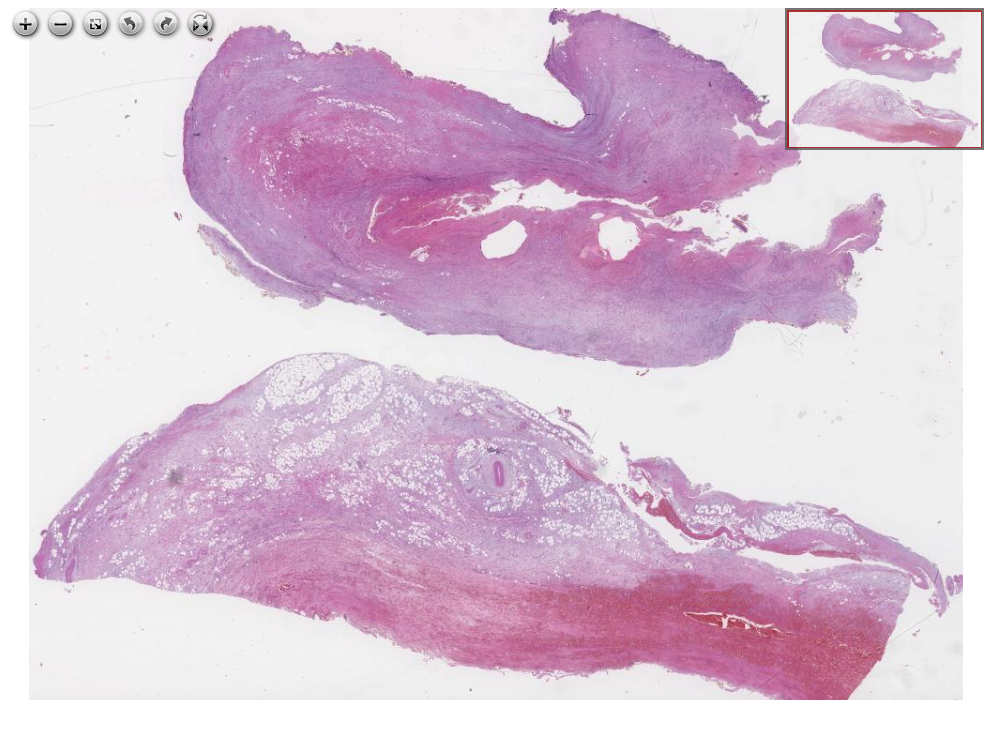
\includegraphics[width=0.25\textwidth,height=\textheight]{./screenshots/thumbnail_fibrosis.png}}
\href{https://images.patolojiatlasi.com/fibrosis/HE.html}{Tam Ekran
Görmek İçin Resmi Tıklayın}

\section{Keloid - Skar}\label{sec-keloid-skar}

Keloid Skar oluşumu


\includegraphics[width=0.15\textwidth,height=\textheight]{index_files/mediabag/qrcodes/keloid-scar-HE_qrcode.pdf}
\href{https://images.patolojiatlasi.com/keloid-scar/HE.html}{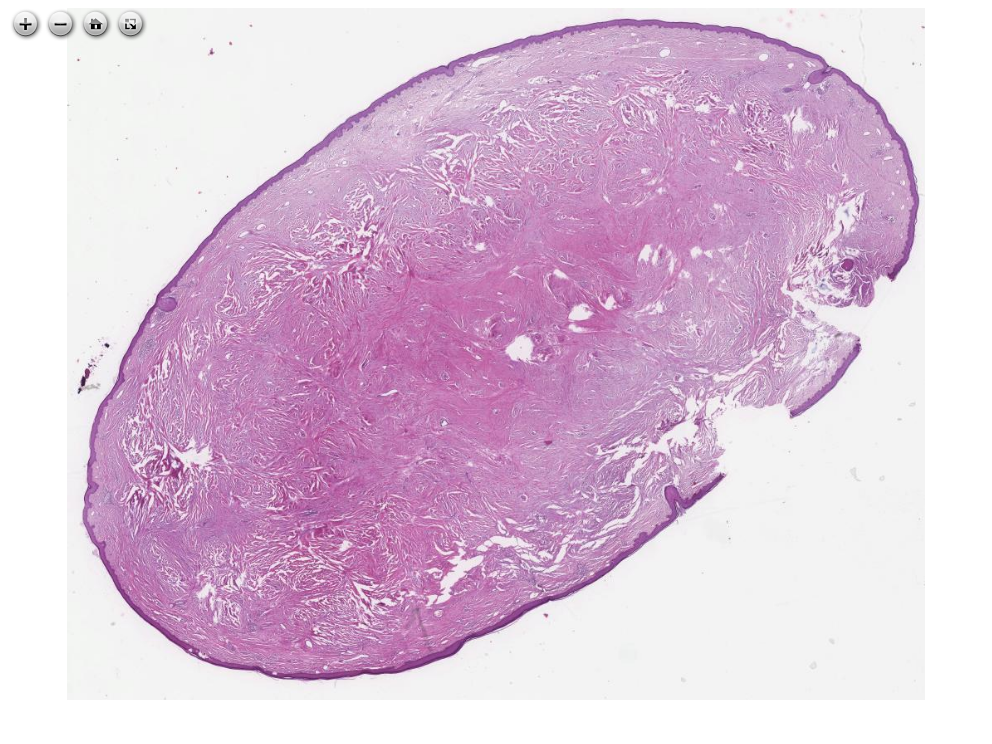
\includegraphics[width=0.25\textwidth,height=\textheight]{./screenshots/thumbnail_keloid-scar.png}}
\href{https://images.patolojiatlasi.com/keloid-scar/HE.html}{Tam Ekran
Görmek İçin Resmi Tıklayın}

Keloid Scar


\includegraphics[width=0.15\textwidth,height=\textheight]{index_files/mediabag/qrcodes/keloid-scar-HE_qrcode.pdf}
\href{https://images.patolojiatlasi.com/keloid-scar/HE.html}{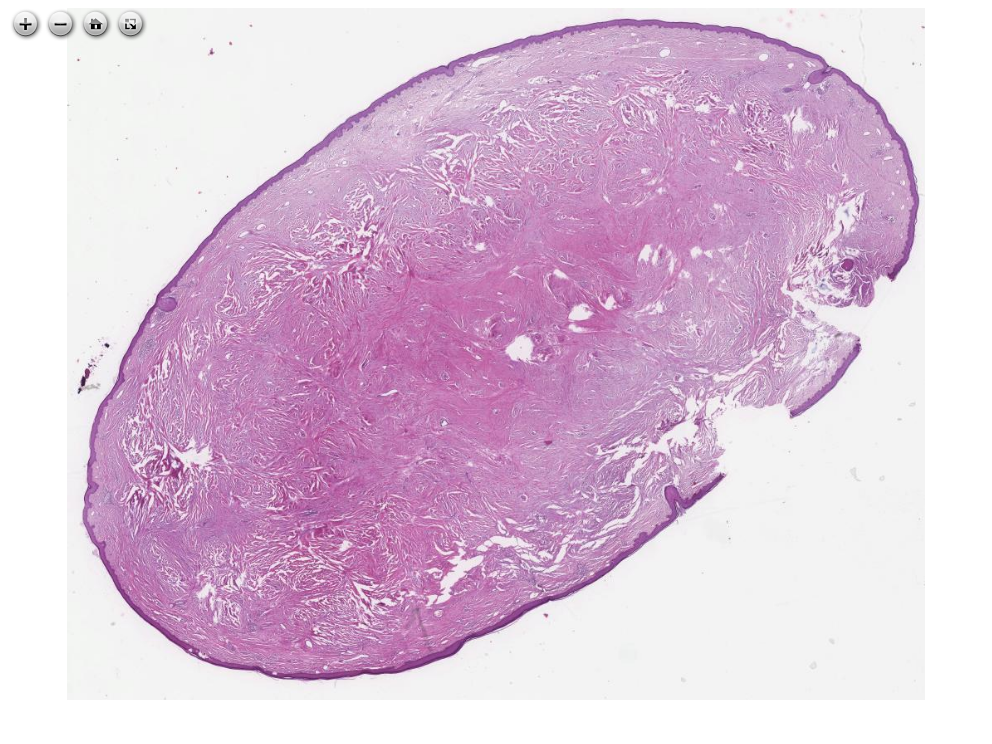
\includegraphics[width=0.25\textwidth,height=\textheight]{./screenshots/thumbnail_keloid-scar.png}}
\href{https://images.patolojiatlasi.com/keloid-scar/HE.html}{Click for
Full Screen WSI}

\chapter{Erozyon}\label{sec-erozyon}

\section{Mide mukozasında erozyon}\label{sec-mide-mukozasinda-erozyon}

\textbf{Mide mukozasında erozyon}


\includegraphics[width=0.15\textwidth,height=\textheight]{index_files/mediabag/qrcodes/erosion-HE_qrcode.pdf}
\href{https://images.patolojiatlasi.com/erosion/HE.html}{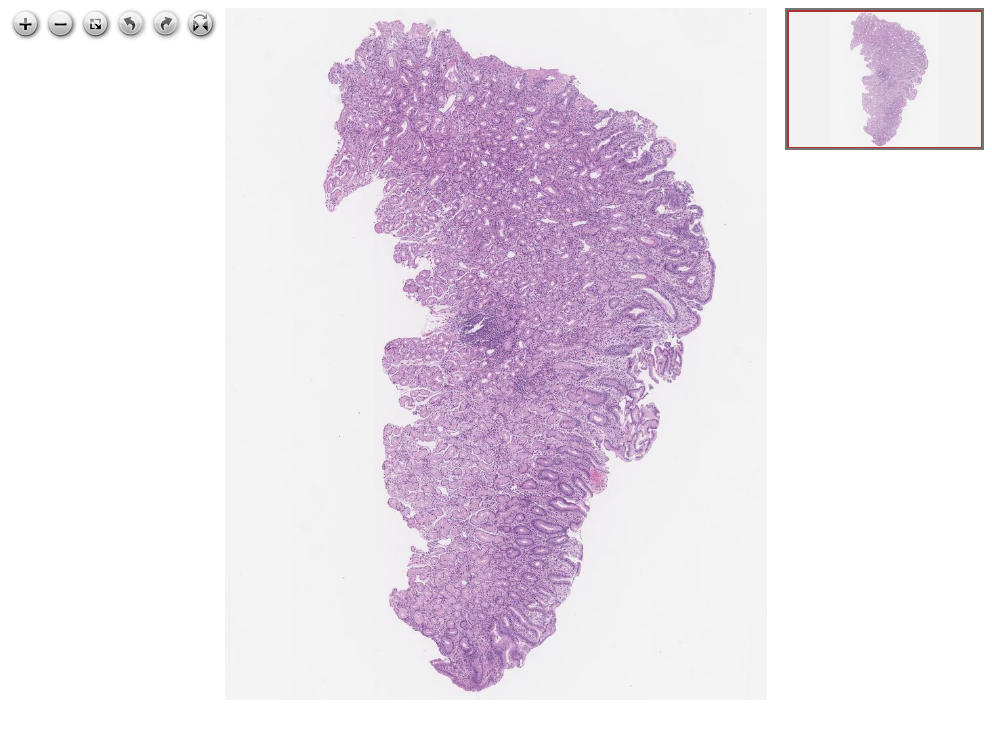
\includegraphics[width=0.25\textwidth,height=\textheight]{./screenshots/thumbnail_erosion.png}}
\href{https://images.patolojiatlasi.com/erosion/HE.html}{Tam Ekran
Görmek İçin Resmi Tıklayın}

\part{İnflamasyon}

\chapter{Akut İnflamasyon}\label{sec-akut-inflamasyon}

\section{Akut Appendisit}\label{sec-akut-appendisit}

\subsection{HE}\label{he-4}

\textbf{Akut appendisit}


\includegraphics[width=0.15\textwidth,height=\textheight]{index_files/mediabag/qrcodes/acute-appendicitis-HE_qrcode.pdf}
\href{https://images.patolojiatlasi.com/acute-appendicitis/HE.html}{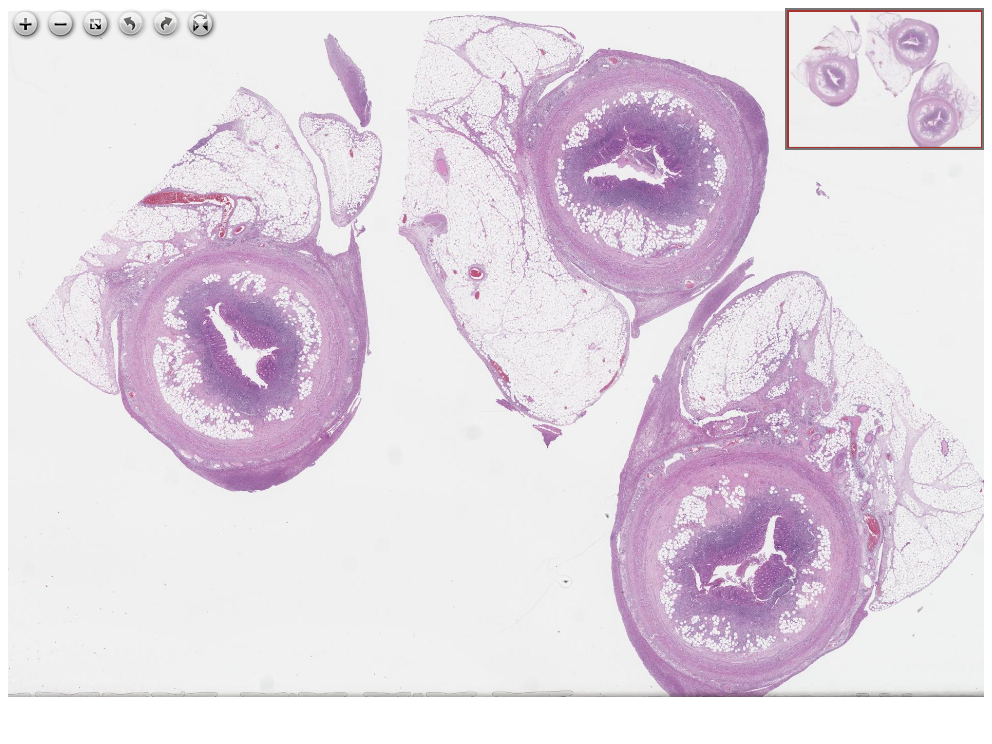
\includegraphics[width=0.25\textwidth,height=\textheight]{./screenshots/thumbnail_acute-appendicitis.png}}
\href{https://images.patolojiatlasi.com/acute-appendicitis/HE.html}{Tam
Ekran Görmek İçin Resmi Tıklayın}

\chapter{Kronik İnflamasyon}\label{sec-kronik-inflamasyon}

\section{Hidronefroz ve Kronik
Pyelonefrit}\label{sec-hidronefroz-kronik-pyelonefrit}

\subsubsection{HE-1}\label{he-1-2}

\textbf{Hidronefroz ve Kronik Pyelonefrit}


\includegraphics[width=0.15\textwidth,height=\textheight]{index_files/mediabag/qrcodes/chronicpyelonephritis-HE1_qrcode.pdf}
\href{https://images.patolojiatlasi.com/chronicpyelonephritis/HE1.html}{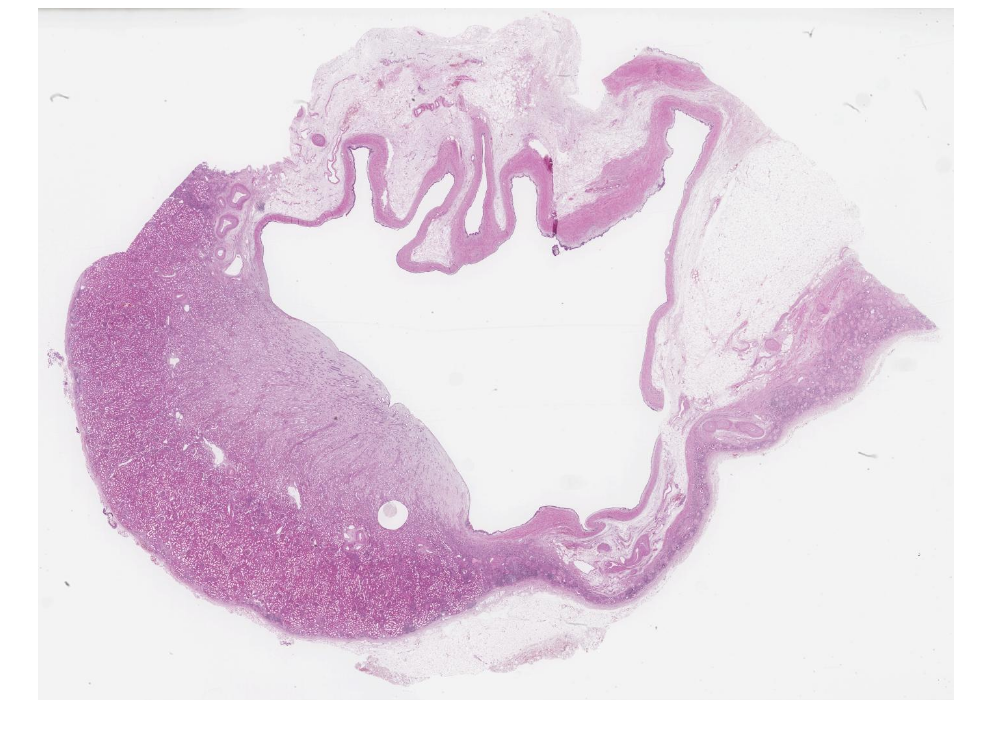
\includegraphics[width=0.25\textwidth,height=\textheight]{./screenshots/thumbnail_chronicpyelonephritis-1.png}}
\href{https://images.patolojiatlasi.com/chronicpyelonephritis/HE1.html}{Tam
Ekran Görmek İçin Resmi Tıklayın}

\subsubsection{HE-2}\label{he-2-2}

\textbf{Hidronefroz ve Kronik Pyelonefrit}


\includegraphics[width=0.15\textwidth,height=\textheight]{index_files/mediabag/qrcodes/chronicpyelonephritis-HE2_qrcode.pdf}
\href{https://images.patolojiatlasi.com/chronicpyelonephritis/HE2.html}{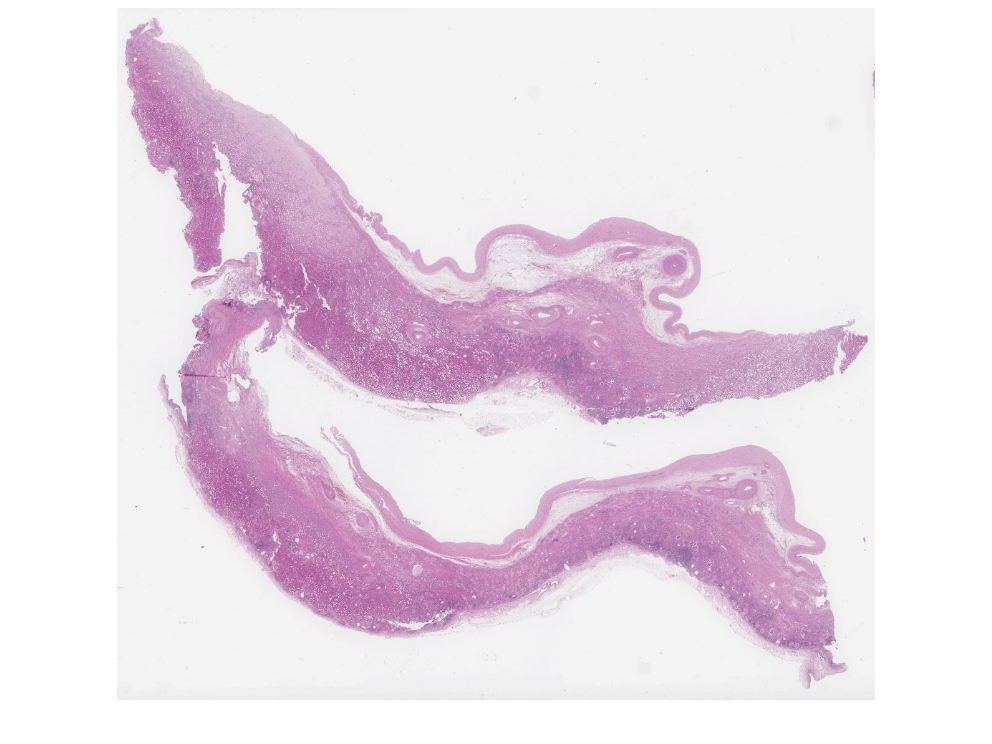
\includegraphics[width=0.25\textwidth,height=\textheight]{./screenshots/thumbnail_chronicpyelonephritis-2.png}}
\href{https://images.patolojiatlasi.com/chronicpyelonephritis/HE2.html}{Tam
Ekran Görmek İçin Resmi Tıklayın}

\subsubsection{HE-1}\label{he-1-3}

\subsubsection{HE-2}\label{he-2-3}

\section{Kronik Pyelonefrit}\label{sec-kronik-pyelonefrit}

\textbf{Kronik Pyelonefrit}


\includegraphics[width=0.15\textwidth,height=\textheight]{index_files/mediabag/qrcodes/chronic-pyelonephritis-HE_qrcode.pdf}
\href{https://images.patolojiatlasi.com/chronic-pyelonephritis/HE.html}{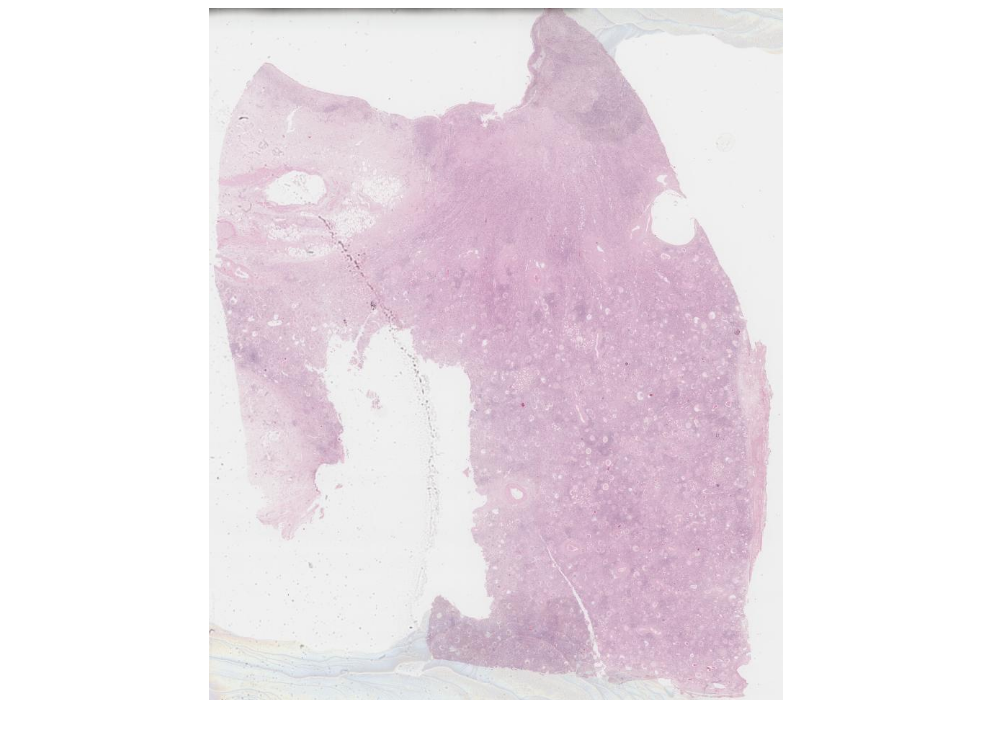
\includegraphics[width=0.25\textwidth,height=\textheight]{./screenshots/thumbnail_chronic-pyelonephritis.png}}
\href{https://images.patolojiatlasi.com/chronic-pyelonephritis/HE.html}{Tam
Ekran Görmek İçin Resmi Tıklayın}

\chapter{Granülom}\label{sec-granulom}

\section{Granülomatöz İnflamasyon}\label{sec-granulomatoz-inflamasyon}

\subsection{Nekrotizan Granülamatöz
İnflamasyon}\label{sec-nekrotizan-granulamatoz-inflamasyon}

\textbf{Karaciğer dokusunda nekrotizan granülamatöz inflamasyon}


\includegraphics[width=0.15\textwidth,height=\textheight]{index_files/mediabag/qrcodes/necrotisinggranuloma-HE_qrcode.pdf}
\href{https://images.patolojiatlasi.com/necrotisinggranuloma/HE.html}{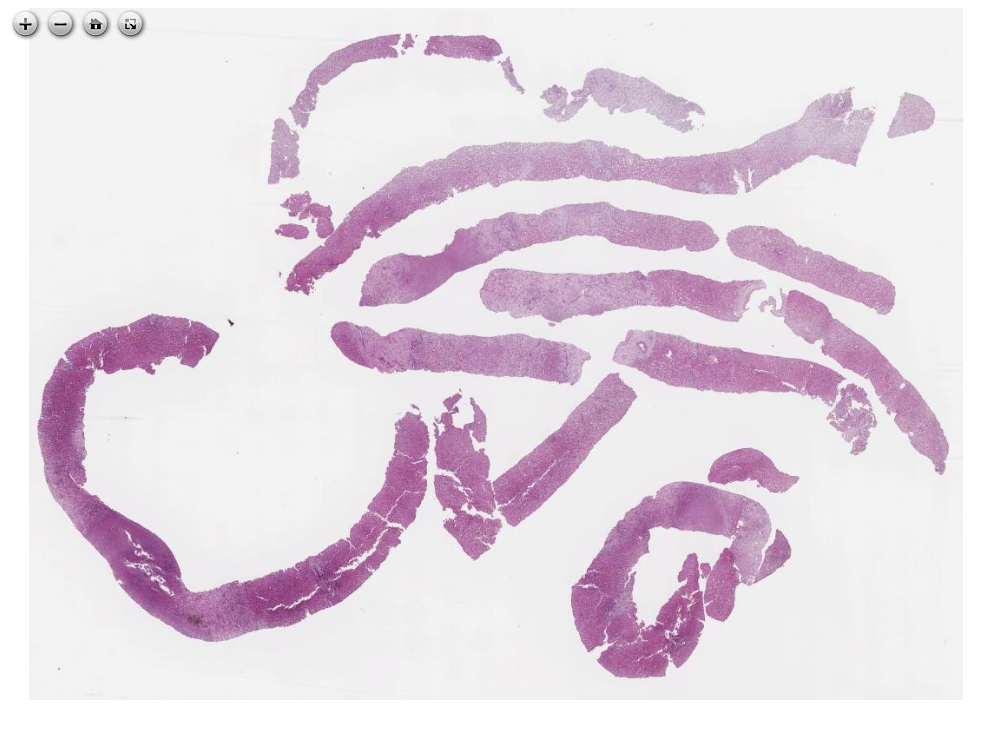
\includegraphics[width=0.25\textwidth,height=\textheight]{./screenshots/thumbnail_necrotisinggranuloma.png}}
\href{https://images.patolojiatlasi.com/necrotisinggranuloma/HE.html}{Tam
Ekran Görmek İçin Resmi Tıklayın}



\end{document}
